%
%  $Author: ienne $
%  $Date: 1995/09/15 15:20:59 $
%  $Revision: 1.4 $
%

% \documentclass[10pt,journal,cspaper,compsoc]{IEEEtran}   %%%tc version
\documentclass[10pt, conference]{IEEEtran}
%\documentclass[conference,compsoc]{IEEEtran}
%\documentclass[10pt, conference]{IEEEtran}
%\documentclass[times, 10pt,onecolumn]{article}
\usepackage{amsmath, amssymb, enumerate}

%%%%%%%%%%%%%%%% page control%%%%%%%%%%%%%%%%%
%\usepackage[margin=0.75in]{geometry}

%\linespread{0.991}  %%%%%%%%%%%%%%%%%%%%%%%%%%%%%%%%% this is really useful
%\usepackage{cite}
\usepackage{fancybox}
\usepackage{amsfonts}
%\usepackage{algorithm}
%\usepackage[noend]{algorithmic}
\usepackage[usenames]{color}
%\usepackage{colortbl}
%\usepackage[ figure, boxed, vlined]{algorithm2e}
%\usepackage[linesnumbered,vlined]{algorithm2e}
%\usepackage[lined,boxed]{algorithm2e}
\usepackage{listings}

\usepackage[linesnumbered,vlined]{algorithm2e}
\usepackage{graphicx}
\usepackage{times}
\usepackage{psfrag}
\usepackage{subfigure}
\usepackage{caption}
%\usepackage{subcaption}
\usepackage{multirow}
%\usepackage{setspace}
%\usepackage{listings}
\usepackage{epsfig}
%\usepackage{epstopdf}
%\usepackage[font=small,labelfont=bf]{caption}
\usepackage{url}

\usepackage{color}
\def\fixme#1{\typeout{FIXED in page \thepage : {#1}}
%\bgroup \color{red}{} \egroup}
\bgroup \color{red}{[FIXME: {#1}]} \egroup}


%\usepackage[pdftex]{hyperref}
\usepackage{rotating,tabularx}

\interfootnotelinepenalty=10000

%% Define a new 'leo' style for the package that will use a smaller font.
\makeatletter
\def\url@leostyle{%
  \@ifundefined{selectfont}{\def\UrlFont{\sf}}{\def\UrlFont{\small\ttfamily}}}
\makeatother

%\documentstyle[times,art10,twocolumn,latex8]{article}

%-------------------------------------------------------------------------
% take the % away on next line to produce the final camera-ready version
\pagestyle{plain}
%\thispagestyle{empty}
%\pagestyle{empty}

\newtheorem{theorem}{Theorem}
\newtheorem{lemma}[theorem]{Lemma}

%% remaining budget share, used in task stall section.
\newcommand{\bottomrule}{\hline}
\newcommand{\toprule}{\hline}
\newcommand{\midrule}{\hline}
%-------------------------------------------------------------------------
\begin{document}

\title{DeepPicar:​ ​A​ ​Low-cost​ ​Deep​ ​Neural​ ​Network-based​ ​Autonomous​ ​Car}
\author{Author One, Author Two\\
\{author1,author2\}@ku.edu\\
University of Kansas, USA\\ 
}

\maketitle
\thispagestyle{empty}
\begin{abstract}

Abstract goes here.

\end{abstract}

%-------------------------------------------------------------------------

%% UPenn's f1/10 BOM: $3,628.37	
%% http://f1tenth.org/
%% http://selfdrivingcars.mit.edu/
%% http://fast.scripts.mit.edu/racecar/
%% https://github.com/mit-racecar

\section{Introduction}
Autonomous vehicles have been a topic of increasing interest in many
disciplines in recent years. Due to the nature of autonomous vehicles,
it is necessary that all real-time operations are successfully
performed prior to their deadlines. This requires that the AV platform
be capable of completing all necessary computations in a timely
manner, while maintaining a high level of accuracy. Consequently, the
cost of creating a platform capable of self-driving can be relatively
high, especially in the current cost-sensitive climate of the
automotive industry \cite{}. The overall price for an autonomous
vehicle platform currently acts as a bottleneck, especially from an
academic standpoint, where cost is an important factor. For many
researchers and students, the charge associated with autonomous
vehicle research is a significant barrier. These same parties may also
be deterred from participating in autonomous vehicle research due to
the potential for their developed platforms to break in the
experimental process. The idea of building one relatively expensive
platform may not be too daunting for some, but the notion of
potentially making multiple identical platforms in case of accidents
may be overwhelming. Toward this end, we explore the possibility of
developing a low-cost system that still employs state-of-the-art AI
technologies and is capable of executing real-time autonomous vehicle
operations. 
	
In this paper, we present DeepPicar, a low-cost autonomous car
platform for research and education. From hardware perspective, 
DeepPicar is comprised of a Raspberry Pi 3 Model B quad-core
computer, a web camera and a RC car, all of which are affordable
components (less than \$200 in total).
The DeepPicar, however, employs state-of-the-art AI
techonologies, including a vision-based end-to-end control system that
utilizes a deep convolutional nueral network (CNN).
The network receives an image frame from a single forward
looking camera, as input and generates a predicted steering angle
value as output at each control period in \emph{real-time}. 
The network is deep as it has 9 layers, about 27 million connections
and 250 thousand parameters (weights).
The network architecture is in fact identifical to the one
used in Nvidia's DAVE-2 self-driving car~\cite{Bojarski2016}. Other
than the obvious difference in scale (RC car vs. real car), from the
computing perspective, the only differences between
the two systems are that our system is implemented in
TensorFlow~\cite{abadi2016tensorflow} and runs on a 
Raspberry Pi 3 whereas Nvidia's DAVE-2 systems is implemented in Torch
7~\cite{collobert2011torch7} and runs on a Drive PX computer (NVIDIA's
automotive specialized computing system~\cite{drivepx}), which is more
powerful but also more expensive.

We follow the standard supervised learning methodology to train the
system with a goal of following lanes on the ground, mimicking real
roads. We first collected data for taining and validation by manually 
controlling the RC car and recording the vision (from the webcam
mounted on the RC-car) and the human control inputs. We then train the
network offline using the collected data on a desktop computer, which
equips a Nvidia GTX 1060 GPU. Finally, the trained network is copied
back to the Raspberry Pi, which is then used to perform interference
operations---locally on the Pi---in the car's main control loop in
real-time. For real-time control, each \emph{inference} operation must
be completed within the desired control period. (e.g., 50ms period for
20Hz control frequency.)

The primary {\bf contributions} of this paper are as follows:
\begin{itemize}
  \item We present the design, implementation, and case-study of a low-cost
    autonomous vehicle that utilizes the state-of-the-art aritificial 
    intelligence techniques.
  \item We systematically analyze real-time characteristics of
    multiple embedded computing platform, including the Raspberry Pi 3
    Model B, in the contex of a vision-based autnomous driving.
\end{itemize}

%% We chose to use a Raspberry Pi 3 not only because of its
%% affordability and availability but also because it is representative
%% of today's mainstream low-end multicore processors, found in
%% smartphones, tables and other embedded devices.
%% The DeepPicar is comprised of a Raspberry
%% Pi 3 Model B, a camera and a low cost RC car.

%% By creating and using the Picar platform, we seek to accomplish the 
%% following three goals. First, the significant reduction of the overall
%% cost required 
%% would make autonomous driving research more accessible to interested
%% individuals/parties. Furthermore, it would remove the concerns of
%% creating replacement platforms as each part, or the entire system,
%% could be replaced relatively inexpensively. Second, the utilization of
%% a more cost-efficient platform would allow for a better understanding
%% of the performance requirements necessary for efficiently operating
%% autonomous vehicles. Finally, we strive to achieve the ability to
%% compare the real-time performance of multiple embedded computing
%% platforms. 

%% We display the efficacy of the Picar by training and testing the
%% DeepTesla DNN \cite{} in a custom-made environment. We find that the
%% Picar is capable of consistently accomplishing all real-time
%% operations required for autonomous driving in a 50 millisecond frame. 

The remaining sections of the paper are as follows: Section II gives
an overview of the platform, including the high-level system and the
methods used for training and inference. Section III discusses the
ways/methodologies in which training data was collected. Section IV
outlines the network architecture. This is followed by the real-time
DNN inferencing in Section V. Section VI reviews the online/offline
training done with the platform, with an evaluation given in Section
VII. Section VIII gives a discussion of related works, and the paper
finishes with conclusions in Section IX. 

\section{Background}
Cite a paper \cite{barroso2009datacenter}.

Cite multiple papers \cite{banga99resourcecontainers,barroso2009datacenter}

\section{Platform Overview}
...
\section{Data Collection}
...
\section{Network Architecture}
...
\section{Real-Time DNN Inferencing}
...
\section{Online/Offline Training}
...
\section{Evaluation}
In evaluating the real-time efficacy of the Raspberry Pi 3, the same methodology is utilized in all 
experiments conducted. The performance of the Pi is measured over a set of 1001 video frames that are 
each individually fed to the model. The processing time for the first frame is ignored as, due to 
cache warmup, it is uncharacteristically high and doesn't accurately represent the Pi's capabilities. A 
deadline of 50 ms, or 20 Hz, is used as a baseline to assess the Pi's ability to complete all 
necessary real-time operations in a timely manner. Also, please note that frame processing times 
would be approximately the same if the input stream was a 
camera instead of a video. 

\subsection{Real-Time Operations}
In our platform, three main real-time tasks are performed during autonomous operation. 
In order, those operations are: (1) capturing and reading the input frame from the designated camera 
or video stream, (2) preprocessing the acquired frame so that it is compatible with the DNN, and (3) 
feeding the frame to and getting the angle prediction from the model. However, the time it takes to 
complete each of the operations will differ, with at least one of them being the dominating step in 
processing each frame.

\begin{figure}[h]
  \centering
  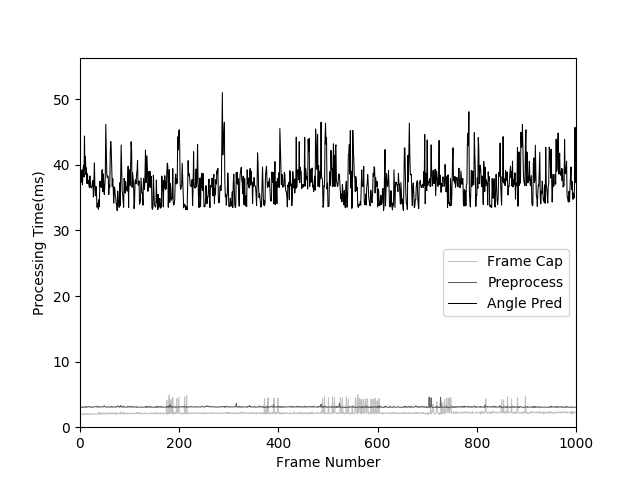
\includegraphics[width=.5\textwidth]{Operation_Time}
  \caption{ Real-time operation completion time in processing frames.}
\end{figure}

In order to determine which operation(s) take the longest to execute, we measured the time it 
took for each step to be completed. For this experiment, all four of the Pi's cpu cores were utilized, 
and only one model was run. As is shown in Fig. 1, the angle prediction operation (3) consumes the 
majority of the processing for each frame. Furthermore, the time it takes for the operation to 
complete is volatile, and can range anywhere between 30 ms and 50 ms for any particular frame. On the 
other hand, both the frame capture (1) and preprocessing (2) operations take substantially less time 
and are relatively more consistent in their times, at 2 ms and 3 ms, respectively. 

\subsection{Multicore Performance}
It may not always be the case that all four cores of the Raspberry Pi 3's Cortex A-53 CPU can be used 
solely for the purpose of operating an autonomous vehicle. Thus, we test how the number of cores 
utilized for real-time operations affects the Pi's overall ability to function as an autonomous 
vehicle platform.

\begin{table*}
  \begin{tabular} {| l | l | l | l | l | l | l | l | l | l |}
    \hline
    \textbf{num cores} & \textbf{mean} & \textbf{max} & \textbf{99.999pct} & \textbf{99.99pct} & 
      \textbf{99.9pct} & \textbf{99pct} & \textbf{min} & \textbf{median} & \textbf{stdev} \\ \hline 
    1 & 61.95813584 & 65.99712 & 65.99277693 & 65.9536558 & 65.562445 & 63.30799 & 59.304 & 61.975479 & 
      0.506466 \\ \hline
    2 & 50.49184 895 & 71.54608 & 71.5404019 & 71.4893194 & 70.978494 & 70.02651 & 46.93723 & 50.011516 & 
      3.162015 \\ \hline
    3 & 48.11392045 & 72.21985 & 72.21789317 & 72.200294 & 72.024303 & 58.44643 & 41.15391 & 48.444033 & 
      4.178325 \\ \hline
    4 & 42.66992688 & 56.36907 & 56.33994633 & 56.0778672 & 53.457076 & 50.70305 & 38.26094 & 42.286992 & 
      2.800991 \\
    \hline
  \end{tabular}
  \caption{Real-time performance of the Raspberry Pi 3 depending on the number of cores used.}
\end{table*}

As is depicted in Table 1, the Raspberry Pi performed better, on average, when it utilized more 
cores. With 4 cores, the Pi was able to meet the vast majority of its 50 ms deadlines, doing so in 
almost 99\% of the processed frames. The Pi had the worst average performance when using only 1 core, 
as it was unable to meet any of the 50 ms deadlines (its fastest processing time was just under 60 
ms). Another observation is that the difference between using 2 cores and 3 cores is relatively 
small. On average, using 3 cores only performed better by 2 ms, so the addition of one core in that 
specific case offers relatively little improvement. However, please note that the average time when 
using 3 cores was below the 50 ms deadline, while the average time using 2 cores was slightly above it. 
One important observation that can be made is that of consistency, as using only 1 core had a much 
steadier performance. As a result, the use of multiple cores is very beneficial in terms of reducing 
the time it takes to complete real-time operations, but may ultimately result in processing times 
that are more volatile.

\subsection{Multimodel Performance}
In a real world scenario, it is highly probable that multiple models will need to be used 
simultaneously in order to perform various important tasks (angle prediction, object detection, 
etc.)\cite{}. As such, we also tested the capability of the Raspberry Pi to run multple models at the 
same time, and measure whether all models are able to meet their respective deadlines on a consistent 
basis. Specifically, the Pi is tested in the cases of running 2 and 4 models simultaneously. For each 
case, all models are allocated an equal number of cores, with 2 models having 2 cores each, and 4 
models having 1 core each.

\begin{table*}[t]
  \begin{tabular} {| l | l | l | l | l | l | l | l | l | l |}
  \hline
  \textbf{num models} & \textbf{cores} & \textbf{mean} & \textbf{max} & \textbf{L1 refs} & \textbf{L1 
    misses} & \textbf{L1 miss \%} & textbf{L2 refs} & \textbf{L2 misses} & \textbf{L2 miss \%} \\ \hline
  1 & 0 &  62.48010421 & 66.83707237 & 27,809,824,750 & 435,932,903	& 1.568 & 2,830,285,204	& 
    358,764,318 & 12.68 \\ \hline
  1 & 0,1 & 51.35843444 & 72.92294502 & 30,354,597,625 &  477,953,407 & 1.575 & 3,308,819,327 & 
    367,823,926 & 11.12 \\ \hline
  2 & 0,1 & 58.03400564 & 83.67586136 & 30,426,714,898 & 490,709,126 & 1.613 & 3,912,431,599 & 
    425,658,305 & 10.88 \\ \hline
  2 & 2,3 & 56.39569068 & 82.88908005 & 30,350,459,058 & 480,166,192 & 1.582 & 3,877,553,207 & 
    421,339,847 & 10.87 \\ \hline
  4 & 0 & 77.90289187 & 104.2420864 & 27,853,570,186 & 452,700,705 & 1.625 & 3,360,219,598 & 
    443,088,325 & 13.19 \\ \hline
  4 & 1 & 78.88618684 & 108.7918282 & 27,868,355,666 & 464,332,042 & 1.666 & 3,415,627,978 & 
    437,962,230 & 12.82 \\ \hline
  4 & 2 & 77.80583382 & 111.9449139 & 27,799,436,982 & 444,828,792 & 1.6 & 3,449,341,398 & 440,580,899 
    & 12.77 \\ \hline
  4 & 3 & 77.86954451 & 99.28488731 & 27,875,785,919 & 445,229,272 & 1.597 & 3,408,895,945 & 
    439,091,391 & 12.88 \\
  \hline
  \end{tabular}
  \caption{Real-time performance of the Raspberry Pi 3 depending on the number of models being run 
    simultaneously.}
\end{table*}

Ideally, each model run would replicate a single model run. However, Table 2 shows that such was not 
the case. In the tests where 2 models ran simultaneously, both of the models showed average time 
increases of around 5-7 ms, around 10\%, when compared to a baseline of 1 model running on two cores. 
This change, however, did not seem to be caused by any form of cache interference as both L1 and L2 
cache misses remained constant, regardless of the number of models running. The number of L1 misses 
being close to 1.6\% of all references and the number of L2 misses being about 11\% of all 
references.

The difference was even greater in the case of 4 models running concurrently, as each one displayed 
an average time increase of approximately 15 ms, around 30\%, when compared to a single model 
running on 1 core. Once again, though, cache interference was not a factor as the number of L1 cache 
misses remained 1.6\% of all references, and the number of L2 cache misses stayed at 13\% of all 
references.

\subsection{Performance Requirements}
In the utilization of the Raspberry Pi 3 in our platform, there are a few factors that need to be 
considered and/or enforced in order to guarantee that the Pi is able to consistently perform at a 
desired level. Specifically, these issues all have the potential to negatively affect the cpu clock 
speed/frequency, which would result in decreased performance. While, in the above experiments, the cpu 
operated at a preferred clock speed of 1.2 GHz, it is entirely possible for the cpu to operate at a 
lower frequency if the following problems are not taken into account.

The most notable issue that can affect the cpu clock speed is that of the power supplied to the 
Raspberry Pi. In essence, it is necessary that the Pi be supplied with 2 Amps, as any less could 
hinder the Pi's ability to maintain a 1.2 GHz frequency. In experiments done with a power supply that 
only provided 1 Amp, the Pi was unable to sustain a 1.2 GHz clock speed and, instead, fluctuated 
between operating at 600 MHz and 1.2 GHz. As a result, it is necessary, or at least highly 
recommended, that the power supply used for the Raspberry Pi 3 be capable of outputting 2 Amps, 
otherwise optimal performance isn't guaranteed.

Another factor that can affect clock speed is that of the cpu's temperature. Some model operations can 
be computationally intensive, thus it is possible for the temperature of the cpu to become relatively 
high. This can be especially problematic in situations where multiple models are running 
simultaneously on the Pi. As a consequence, thermal throttling may be used to decrease the clock 
speed so that the cpu temperature stays at a safe level. As such, the Raspberry Pi may not be suited 
for prolonged use, especially in cases where the workload is relatively larger, like running multiple 
models. Rather, the Pi seems to be better suited for running in set periods, after which it is turned 
off or made idle so that the cpu is given time to cool down.
\section{Related Work}
\cite{Bojarski2016}

\section{Conclusion}
%-------------------------------------------------------------------------

\bibliographystyle{plain}
\bibliography{reference}
\end{document}
